\section{Implementation}\label{sec:implementation}

The following subsections describe the implementation of the design explained in the previous section. The conceptual data model from section~\ref{sec:conceptual_model} is translated to Clojure in section~\ref{sec:impl_datamodel}. Next, a guided tour follows the \emph{data path} from a new fact originating on a client all the way through the server and to the other clients, showing and explaining the simple functions that transform it along the way.

\paragraph{Functional core, stateful shell.}
While Clojure does not enforce functional purity, it is idiomatic to push impure computation and state towards the edge of the system. In fact, core functionality described in the next subsection is implemented as pure functions operating on plain immutable data structures. Such purity allows the same core of the database to run unmodified on servers and on clients. Clients and server obviously need to keep some state, but each does so within one single place only. Three pure namespaces make up the functional core of the system:

\begin{enumerate}[label={(\roman*)}]
  \item \lisp{core} implementing the basic pure functions and data structures to create and transact facts,
  \item \lisp{index} implementing pure functions to place facts into indices,
  \item \lisp{query} implementing pure functions to provide basic querying capabilities with a language based on edn Datalog.
\end{enumerate}

The minimal impure parts stay within the \lisp{client} and \lisp{server} namespaces. Their task is to handle the asynchronous connection with each other (\lisp{connect!}, \lisp{disconnect!}, \lisp{receive}, \lisp{broadcast!}) and mutate their local copy of the database (\lisp{transact!})


\cleardoublepage
\begin{figure}[!ht]
  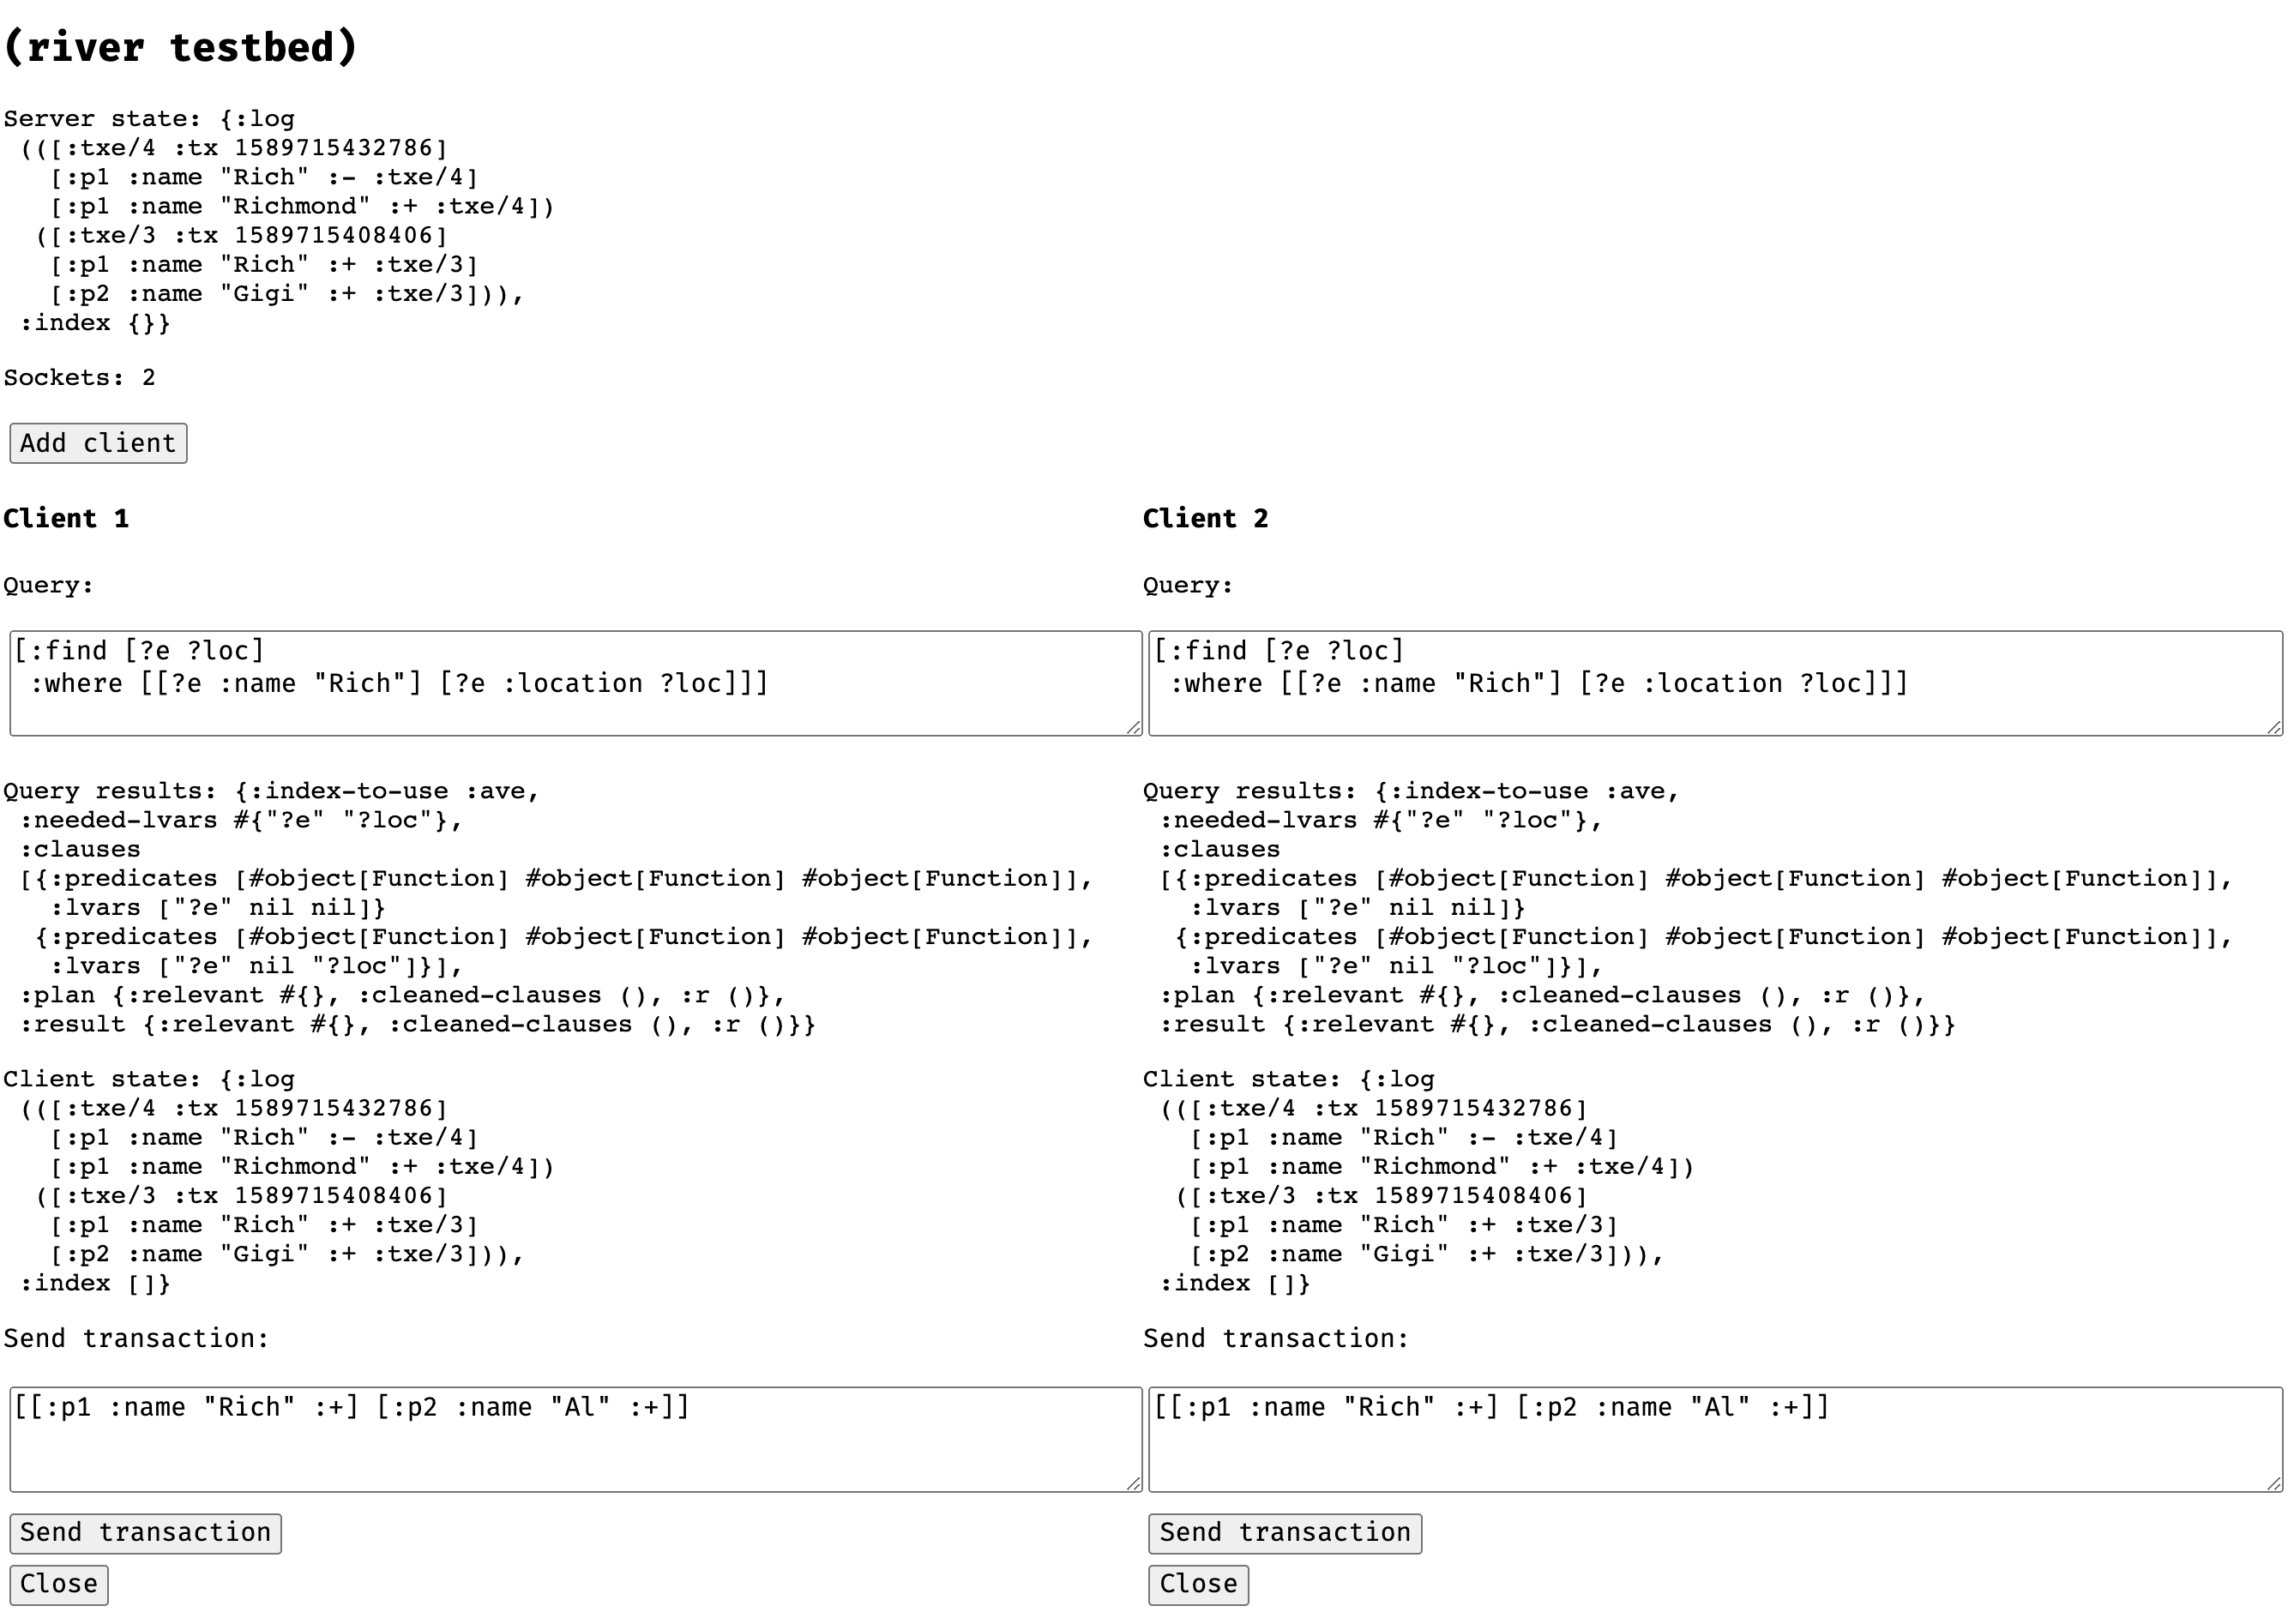
\includegraphics[width=\linewidth]{images/testbed.png}
  \caption{Two connected clients in the testbed}
  \label{fig:testbed}
\end{figure}

\paragraph{The testbed.} To aid quick experimentation while developing, all interactions between the server and the clients are simulated within a single web page. The scaffolding in the \lisp{testbed} namespace presents a simple UI to add and remove client connections, to transact facts, and to perform queries, all while providing insight into the full current state of each simulated node, see figure~\ref{fig:testbed}. The testbed can inject arbitrary delay into Clojure's \lisp{core.async} \emph{channels} used to simulate WebSocket connections between nodes. The channels implementation of the testbed is based on \cite{ittyon}.


\cleardoublepage

\subsection{Data model}\label{sec:impl_datamodel}
The implementation relies heavily on the lazy immutable default data structures \cite{hickey2009persistent} provided by the Clojure core library, which remain performant even when used in strange ways thanks to structural sharing \cite{okasaki1999purely}. This section extends and clarifies the design from section~\ref{sec:conceptual_model} and translates it into Clojure.

\begin{itemize}
\item A \emph{fact} is represented as a vector, its elements can be of any Clojure value type.

\begin{center}
  \lisp{[e a v]}
\end{center}

\item A \emph{transition} is either an \emph{assertion} or \emph{retraction}, a vector containing the splatted fact as its first three elements, along with an indicator whether to assert (\lisp{:+}) or retract (\lisp{:-}) the preceding fact.

\begin{center}
  \lisp{[e a v :+]}
\end{center}

\item A \emph{transaction} is a vector containing an arbitrary number of transitions, which are to be atomically applied to the log \emph{at some point in the future.} Note that a transaction does not mutate the database, it is at this point just a data structure expressing intent to assert or retract facts. A transaction may contain \emph{meta facts} about itself, using the "magic" placeholder value for the transaction entity \lisp{:tx-meta}.

\begin{center}
  \lisp{[[e a v :-] [e a v :+] [:tx-meta a v :+]]}
\end{center}


\item A \emph{commit} (listing~\ref{lst:commit_structure}) is a transaction that was successfully applied to the database, meaning that any consistency criteria succeeded and a new database value containing the updated state was produced. It has similar shape and contents as the transaction it represents. Each transition of the committed transaction contains as its last element the same newly-generated transaction entity reference \lisp{txe}. There is also now at least the $t_x$ transaction meta fact added and optionally any derived facts.

\begin{lstlisting}[label={lst:commit_structure},morekeywords={:+,:-,txe},caption=Structure of a commit]
  [[e a v :+ txe]
   [e a v :- txe]
   [txe :$t_x$ $t_x$ :+ txe]]
\end{lstlisting}

\item The \emph{log} is an ordered linked list of all commits. All changes over time to the database are fully described by the log, with the newest commit being appended to the beginning: \lisp{'([...] [...] ...)}.

\cleardoublepage
\item An \emph{index} (listing~\ref{lst:index_structure}) is an associative nested structure (map). There are four indices, each three layers deep: \lisp{:eavt}, \lisp{:veat}, \lisp{:avet}, named after the nesting order of their keys with the last \lisp{t} referring to the transaction entity \lisp{txe}.

\begin{lstlisting}[label={lst:index_structure},morekeywords={:+,:-,txe},caption=Structure of the indices]
{:index
  {:eavt {e {a {v txe}}
          e {a {v txe}} ...}
   :aevt {a {e {v txe}}
          a {e {v txe}} ...}
   :avet {a {v {e txe}}
          a {v {e txe}} ...}
   :vaet {v {a {e txe}}
          v {a {e txe}} ...}}}
\end{lstlisting}

\item Finally, the \emph{database} (db) is a map containing the log list and the index map.

\begin{center}
  \lisp{\{:log '() :index \{\}\}}
\end{center}

\end{itemize}

\paragraph{Commits do not mutate the database.}
Note that a commit itself has no notion of place or state, and does not mutate anything, it only signifies that a transaction was successfully applied to \emph{some} database value \emph{somewhere}. A commit \emph{may} mean that the server has successfully updated its state and broadcast the commit to all connected clients, or, since the database value is immutable, it may just be the result of any local \emph{"as-if"} dry run.

\paragraph{Transaction meta facts.}
A client may supply arbitrary transaction metadata, except $t_x$ which is always set by the server. To send metadata, the client adds transitions to the transaction, which have the magic value \lisp{:tx-meta} set as their entity. Before committing a transaction, the server will replace this value in the transitions with a newly generated entity.

\cleardoublepage
\subsection{Writing}

This subsection follows a simple fact in canonical EAV format, originating on a client, through its transformations until it ends up on the server's canonical source-of-truth database. Starting with the fact

\begin{center}
  \lisp{[:patient/91 :name "Hye-mi"]}
\end{center}

and calling \lisp{assert} on it yields an \emph{assertion transition}, which is created through \emph{conjoining} (appending as last element) the \lisp{:+} keyword with the fact vector. Similarly, calling \lisp{(retract fact)} conjoins \lisp{:-}. The result, the example case, is an assertion vector:

\begin{center}
  \lisp{[:patient/91 :name "Hye-mi" :+]}
\end{center}

The database only accepts transitions to be atomically applied as part of a transaction vector. For example, to update a value, simultaneously retract the previous value and assert a new value for the same combination of entity. The variadic \lisp{transact} function only applies its arguments to \lisp{vector}, creating a transaction vector:

\begin{center}
  \lisp{[[:patient/91 :name "Hye-min" :-] [:patient/91 :name "Hye-mi"  :+]]}
\end{center}

\paragraph{On cardinalities.} What would happen if one were to assert multiple values for the same combination of entity and attribute? Should any previous values be retracted automatically, resulting in one value being "true" at a time? Should all values stay current until retracted? The path chosen in this implementation was to only support the more general case of \emph{defaulting to multi-valued cardinalities on all attributes} (which also happens to be simpler to implement). This may lead to unexpected results in queries. A production system would need to define a schema and enforce cardinalities of \emph{many} or \emph{one} on each attribute depending on the requirements of the domain model.

\paragraph{Server interface.}
This transaction can now be committed to a database value, either locally to create a new database (sometimes also referred to as a "what-if" transaction, as it does not affect the value on the server), or globally for all clients by transacting on the server. In production systems, a server should likely not accept arbitrary transactions from clients. Instead, the database is protected by regular \gls{RPC} / REST endpoints which, after authentication, authorization, and sanitization accept only specific parameters to transact.

The testbed server accepts one type of message, a vector beginning with the keyword \lisp{:transact} containing the entire transaction vector nested as its second element:

\begin{center}
  \lisp{[:transact [[:patient/91 ... :-] [:patient/91 ... :+]]]}
\end{center}

When such a transaction message is received, the server applies the transaction and afterwards swaps the global state atom (atomically mutates the reference via a call to \lisp{swap!}) to the new database value. Clients do not attempt to \emph{optimistically} update their local database but rather wait for the server to confirm the transaction and broadcast the final \emph{commit} back to all clients. Safe means for performing optimistic updates remain a topic that needs further research. Clients simply listen to a message tagged \lisp{:commit} and upon receipt proceed to swap their local database value. Be aware that the server may send different commits to each client, depending on their subscription query (explained later in subsection \ref{sec:pubsub_impl}).

\paragraph{ACID transactions.}
Thanks to Clojure's immutable data structures, implementing transactions that respect \gls{ACID} guarantees is almost trivial.
The pure function \lisp{(transact db transaction txe now)} takes a database value, a transaction vector, a new unique entity \lisp{txe} and the current time which is to be used as transaction time $t_x$. The \lisp{txe} value is usually either a globally incrementing number or a randomly generated string like a \gls{UUID} version 4. It is up to the impure calling code on the server to generate and supply these two values. The \lisp{transact} function returns a \emph{new} database value with the transaction committed, i.e. appended to the log and with the indices updated. Transacting is a nested multi-step process:

\begin{itemize}
  \item \lisp{commit}: Generates another data structure which describes the commit about to happen. The same arguments as to \lisp{transact} are passed along, resulting in the commit data structure depicted in listing~\ref{lst:commit_example}:

  \begin{lstlisting}[label={lst:commit_example},morekeywords={:txe/1},caption=A commit of one retraction and two assertions]
      [[:patient/91 :name "Hye-min" :- :txe/1]
       [:patient/91 :name "Hye-mi" :+ :txe/1]
       [:txe/1 :$t_x$ $t_x$ :+ :txe/1]]
  \end{lstlisting}

  To generate this data structure, \lisp{commit} performs the following steps:
  \begin{itemize}
    \item \lisp{(conj transaction [txe :$t_x$ now :+])}: Conjoins the non-optional assertion of the $t_x$ meta fact with the supplied transaction vector.

    \item \lisp{(map #(conj \% txe) transaction)}: Conjoins the \lisp{txe} value as the last element of each transition in the amended transaction vector returned from the previous step.

    \item \lisp{(derive-transitions transaction db txe now)} Some previously added facts in the database may be of a special attribute which indicates that the value is a \emph{derivation function}. These functions receive a pending database value and may return additional assertions or retractions, for example to keep a phonetic index on people's names updated. The behavior of \lisp{derive-transitions} is described later.

    \item \lisp{(validate db)} Finally, the pending commit is applied to a new database, and its installed constraint functions are checked. The behavior of \lisp{validate} is described later.
  \end{itemize}

  \item \lisp{apply-commit}: When the previous steps generated a description of a commit, the last step is to apply the commit: Append it to the log and update all indices. Since the commit being applied was generated from the same basis value of the database, it is guaranteed that all consistency criteria are honored and that this call cannot produce an invalid database.
\end{itemize}

\paragraph{Derivation functions.} Functions are first-class values in any functional language, even more so in a Lisp where all code is represented as data structures, and all data structures can be evaluated as code -- and passed around and stored in the database. These affordances allow the database to \emph{react to changes to itself, on itself}, without side effects.

Users can transact \emph{derivation functions} into the database, which are just facts with the special \lisp {:db/derive} attribute and a function as a value. This function must have the signature:

\begin{center}
  \lisp{($\lambda$ [db commit])}
\end{center}

In the process of creating a commit these derivation functions receive the value of the database and the most current accumulated value of the commit being generated. They are expected to return a \emph{transition vector}, of which any transitions returned will be added to the current commit, before the updated commit vector is passed on to the next derivation function.

Derivation functions cannot mutate the commit vector, but may issue \emph{immediate} retractions of facts contained therein. The order in which installed functions are evaluated is not specified. Since there is no way to enforce functional purity, and they may, but are not recommended to, have side effects.

\paragraph{Consistency constraints.} Enforcing consistency of the database after all derivation functions have been evaluated is similarly trivial to implement: All current facts with a \lisp{:db/validate} attribute have as their value a function with the same signature as derivation functions. For the transaction to commit, every validation function is expected to signal consistency by returning \lisp{true}.

Note that there are no constraints which need to be \emph{disabled} during a transaction, but rather the final database value (after deriving facts and adding them to the current commit) is checked for consistency just once.


\paragraph{Indexing.} The four indices \lisp{:eavt}, \lisp{:aevt}, \lisp{:avet}, and \lisp{:vaet} are created by \emph{folding} over the reversed commit log. Listing~\ref{lst:index_code} shows the entirety of the indexing logic. Transaction boundaries are irrelevant because creating the index is atomic anyways, so the reversed log is flattened before being passed to the fold. Updating an index happens after a commit is finalized, and has the fundamental property of being \emph{incremental}, meaning that to update an existing index, only the newest commit needs to be folded in with the existing index.

The fold is implemented as a reducing function with the database value as its initial element, and with \lisp{index} as its combining function, thus folding one commit into the index at a time.

The \lisp{index} function destructures each element of the commit vector into its sub-elements, and decides the updating function to use based on whether it is an assertion (then associate \lisp{txe} along the index path given by \lisp{e a v}) or a retraction (then dissociate). This is why building the index needs to happen in reverse order of the log. Even though the design of the system selected four common indices to cover general querying use cases, it is a trivial one-line change to the implementation of the \lisp{index} function given in listing~\ref{lst:index_code} to reduce or extend the set of indices to populate. The key to note here is that assertions cause the value of the fact to be \emph{associated in} the index (\lisp{assoc-in}), while retractions dissociate values. The entire index structure, being immutable, is \emph{threaded} ($\rightarrow$) through successive associations to place the value inside each index.

\begin{lstlisting}[label={lst:index_code},morekeywords={:eavt,:avet,:aevt,:vaet,flatten,def,assoc-in,dissoc-in},caption=Updating the index]
(def$\lambda$ index [db [e a v op txe]]
  (update db :index
    ($\lambda$ [index]
      (let [index-in (case op
                       :+ #(assoc-in %1 %2 txe)
                       :- dissoc-in)]
        ($\rightarrow$ index
          (index-in [:eavt e a v])
          (index-in [:aevt a e v])
          (index-in [:avet a v e])
          (index-in [:vaet v a e]))))))

(def$\lambda$ create-index [db]
  (reduce index db
    (flatten (reverse (:log db)))))

(def$\lambda$ update-index [db commit]
  (reduce index db commit))
\end{lstlisting}

Listing~\ref{lst:indexing_example_result} shows the resulting index structures after applying the commit to the database. Note that the retracted fact is not part of the index anymore, it is only accessible by scanning the structured commit log.

\begin{lstlisting}[label={lst:indexing_example_result},caption=Fully populated indices after transacting]
{:index
  {:eavt {:patient/91 {:name {"Hye-mi" :txe/1}}
          :txe/1 {:$t_x$ {$t_x$ :txe/1}}}
   :aevt {:name {:patient/91 {"Hye-mi" :txe/1}}
          :$t_x$ {:patient/91 {$t_x$ :txe/1}}}
   :avet {:name {"Hye-mi" {:patient/91 :txe/1}}
          :$t_x$ {$t_x$ {:txe/1 :txe/1}}}
   :vaet {"Hye-mi" {:$t_x$ {$t_x$ :txe/1}}
          $t_x$ {:$t_x$ {:txe/1 :txe/1}}}}}
\end{lstlisting}



\subsection{Querying}

Now that the fact has been committed to the database on the server, it is time to look at the means available to get answers to questions by querying the database value. Simply looking up data directly via the indices is the preferred way to read. There is no query parsing and execution overhead, since the data is "just here" inside a sorted and easily walkable structure. A developer using this data layer should be familiar with the use cases and performance characteristics of the various indexing structures. Refer to earlier section on the design of the index structure for examples and a comparison of use cases. This subsection sketches the implementation of the edn Datalog query engine, a completely separate and optional library. The implementation is a re-write based on \cite{rubin15aosadb} with macro-heavy code and metadata being replaced by pure functions and maps, among other simplifications. This section will look at the example query in listing~\ref{lst:example_query_2} and trace it through a full evaluation, starting with main entry point, the \lisp{q} function: \lisp{(q db query)}.

\begin{lstlisting}[label={lst:example_query_2},morekeywords={e,name,find,where,room,32},caption="Who's in room no. 32?"]
        [:find [?name]
         :where [[?e :name ?name]
                 [?e :room :room/32]]]
\end{lstlisting}

\paragraph{Step 1: Filter the log by time.}
As per design, nontrivial and performant queries are only supported for the \emph{most recent} view of the database. There is, however, a simple way to trade \emph{some} performance for querying the state at an arbitrary past point of transaction time $t_x$: By constructing a new database value from the current state with its log truncated at some point. More generally, one can also construct a new database out of an arbitrary slice of the log, doing so however may lead to unexpected results because data asserted by "older" facts might be missing as it was cut out in the filtering stage.

\paragraph{Step 2: Build a filtering sieve triple.}

The general working principle of the engine is that each of the \emph{query clauses} is parsed into a \emph{filtering sieve}, that is a vector containing functions which examine each part of the fact and decide whether the value being fed \emph{matches} the expected \emph{data pattern} of the initial clause. In the example, the first query clause: \lisp{[?e :name ?name]} is transformed into the following structure, containing the sieve and a positional mapping back to the logic variable:

\begin{center}
  \lisp{\{:sieve [true #(= \% :name) true] :lvars ["?e" nil "?name"]]\}}
\end{center}

The first nested vector is the sieve. It matches all facts which have an attribute of \lisp{:name}, and it does not care about entity or fact values (\lisp{true} will always match any value in that position). The second nested vector keeps track of the names and positions of the lvars from the supplied query clause, because later, when matching facts are found, their values need to be \emph{unified} with the lvar bindings.

\cleardoublepage
The second query clause is transformed alike:

\begin{center}
  \lisp{[?e :room :room/32]} \\
  \lisp{\{:sieve [true #(= \% :room) #(= \% :room/32)] :lvars ["?e" nil nil]]\}}
\end{center}

The original macro implementation of the query engine by \cite{rubin15aosadb} additionally allows use of any desired unary or binary predicate to be called as part of the matching process by simply wrapping them in a similar sieving function. A production application must take care, e.g. by whitelisting only certain server-side functions as predicates, that clients cannot submit malicious side-effecting code as part of a query. This work borrows the original design from \cite{rubin15aosadb} and simplifies its implementation as in listing~\ref{lst:make-sieve}.


\begin{lstlisting}[label={lst:make-sieve},morekeywords={cond,not,coll,term,lvar,true,t,count,second,first,last,def,make-sieve},caption=Constructing a predicate sieve, adapted from [Rub15]]

(def$\lambda$ make-sieve [term]
  (cond
    ; Logic variables do not filter anything yet
    (lvar? term)
    ($\lambda$ [_] true)

    ; Unary operators must hold: [valid? ?x]
    (and (vector? term)
         (= 2 (count term))
         (lvar? (second term)))
    ($\lambda$ [t] ((first term) t))

    ; Binary operator, lvar is first operand: [> ?age 18]
    (and (vector? term)
         (lvar? (second term)))
    ($\lambda$ [t] ((first term) t (last term)))

    ; Binary operator, lvar is last operand: [< 18 ?age]
    (and (vector? term)
         (lvar? (last term)))
    ($\lambda$ [t] ((first term) (second term) t))

    ; Constants must match exactly
    :else
    ($\lambda$ [t] (= term t))))

\end{lstlisting}


\cleardoublepage
\paragraph{Step 3: Decide index to use.}
The query clauses are now parsed into a sieve which is ready to be evaluated over an index. Descending an index means successively going from knowledge to answer, i.e. evaluation needs to start with an index which has as its top level value one of the constants provided in the query. In other words, the lvar that appears at the same position within each query clause is the \emph{joining variable}. The index which to descend is the one that keeps this joining variable at its leaves \cite{rubin15aosadb}. This is a design limitation, as a full query language should support arbitrary transitive joins, leveraging multiple indices. Refer to table \ref{tbl:lvartoindex} for clarification.

\begin{table}
  \caption{Mapping of joining variable position to query index, slightly adapted from \cite{rubin15aosadb}}
  \begin{tabular}{|r|c|l|}
    \hline
    query clause & joining variable operates on & index to use \\ \hline
    \lisp{[:e :a ?v]} & value & \lisp{:eavt} \\ \hline
    \lisp{[:e ?a :v]} & attribute & \lisp{:vaet} \\ \hline
    \lisp{[?e :a :v]} & entity & \lisp{:avet} \\ \hline
    \end{tabular}
    \label{tbl:lvartoindex}
\end{table}

\paragraph{Step 4: Run sieve function over filtered index}
According to the query design goals, the order of the query clauses has no semantic meaning, yet there is an effect on query evaluation performance: when the most restricting clauses are placed at the beginning, they are processed first and immediately reduce the cardinality of the set of potential results which the next clauses have to filter through. Automatically optimizing clause order would require estimating the cardinality of the resulting sets, which is a complex undertaking and is thus omitted from this proof-of-concept \cite{neumann2011characteristic, malik2007black}.

The \lisp{descend-index} function first needs to \emph{reorder} the sieve functions according to the selected index. Since the sieve is always given in canonical EAV order, before it can be used to descend e.g. an \lisp{:avet} index, the sieve needs to be rearranged so that e.g. the function matching the attribute is moved from second to first position and so on. Actually descending the chosen index is a mechanical iteration, calling each sieve function on its respective index level and accumulating the results.

The result of this sieving process is a \emph{superset} of facts matching \emph{any} of the given query clauses, but with no attention paid to the correct binding and unification of their values with the respective logic variables of the query. The last steps of query resolution are identical to the initial implementation by \cite{rubin15aosadb} and consequently are not further described here.


\cleardoublepage
\subsection{Publishing and subscribing}\label{sec:pubsub_impl}

To keep the implementation of the publication/subscription mechanism simple, a single client only subscribes to one publication at a time. It does so by sending the following message to the server, which causes the submitted query data structure to be \emph{installed} on the client socket:

\begin{center}
  \lisp{[:subscribe query]}
\end{center}

An installed query by itself does not do anything, as it is just a data structure. The server must ensure that whenever its global copy of the database value is \emph{swapped} for an updated value after a successful commit, the interested clients are notified of that commit. To do so, the server walks the list of connected clients and in turn feeds each installed query to the server's \emph{publication function}.

A developer using this data layer in an application needs to set up that custom publication function beforehand. It receives the updated database value and the client's installed query, and is expected to return a \emph{commit} of the changes that should be sent to the client.

Note that the client's queries being passed to the publication function are not expected to be compatible with the described query engine, or be queries at all -- a subscription query can be any data structure, and it is up to the developer using this data layer to supply a publication function which is able to decide, based on the query submitted by the client, what commit should be replicated.

Clients may choose to amend their subscription query at any later point in time by sending a new \lisp{[:subscribe query]} message. A simplistic mapping function from the new database value and the client's current query would not have enough information to decide what parts of the commit need to be replicated, as the client might have initially received some facts pertaining to its initial subscription but has re-subscribed with different parameters in the mean time. The publication function thus may incorrectly assume that the client already has its local database populated with all facts matching the current subscription, whereas the client actually still has all the facts of the previous subscription yet will receive facts for its current one. Consequently, the publication function is also passed the client's previous query, and the transaction entity of the last transaction that was replicated to the client:

\begin{center}
  \lisp{(def$\lambda$ publish [db new-query previous-query last-txe])}
\end{center}

The return value of the publication function is either \lisp{nil} to take no action when the client's subscription is not affected by the latest commit, \lisp{[:commit commit]} to command the client to commit the commit, possibly modified, or, as a last resort if e.g. the query has changed substantially and no diff can reasonably be deduced, the publication function can return \lisp{[:reset log]} to instruct the client to start anew and swap its value to a completely new database created from the attached log. Note that the server never sends index structures over the wire because clients can trivially regenerate them.

\paragraph{Nontrivial publications.}
The publication function may also modify facts, e.g. censor some values matching sensitive attributes or choose to not publish facts matching some pattern. As a consequence of the simplistic notification mechanism, the server may send more or less, or different facts than the client asked for. While the body of the publication function can be trivial and always return the latest commit regardless of query, developers building larger systems will likely need to put a lot of effort into writing an efficient, secure, and correct publication function. The simplistic design of the publication/subscription mechanism appears to be the weakest point of the presented data layer, as it only shifts to the developer almost all of the complexity related to efficiently distributing and diffing results from changed queries.
